\begin{pastexam}[label={px:ntut-114-ee-ds-13}]{北科大電機所（戊組） 114 學年度 第 III-5 題}
（追蹤；20 分）

Read the following array A in the given order and show the corresponding trees:
\begin{center}\texttt{A 20,7,15,4,12,9,11,25,6}\end{center}
(a) Construct a binary search tree for A. Draw the resulting tree. \textbf{(5\%)}\\
(b) Show the post-order sequence of the obtained tree in (a). \textbf{(5\%)}\\
(c) Construct a MIN-heap for these numbers using the Top-Down Strategy. Draw the resulting heap.
\textbf{(5\%)}\\
(d) Show heap sort in ascending order using the MIN-Heap in (c). \textbf{(5\%)}
\end{pastexam}

\begin{pastsoln}
(a)(b) 是二元搜尋樹（資結書第~9~章），(c)(d) 是堆積（第~8~章），本題放在第~8~章。

\textbf{(a)} 依序插入（小的往左、大的往右，走到空位放下）：
\begin{itemize}
\item 20 當根；7 $< 20$ 放左邊；15：$< 20$、$> 7$，放 7 的右邊；4：$< 20$、$< 7$，放 7 的左邊。
\item 12：$< 20$、$> 7$、$< 15$，放 15 的左邊；9：$< 20$、$> 7$、$< 15$、$< 12$，放 12 的左邊。
\item 11：$< 20$、$> 7$、$< 15$、$< 12$、$> 9$，放 9 的右邊；25 $> 20$，放 20 的右邊。
\item 6：$< 20$、$< 7$、$> 4$，放 4 的右邊。
\end{itemize}
\begin{center}
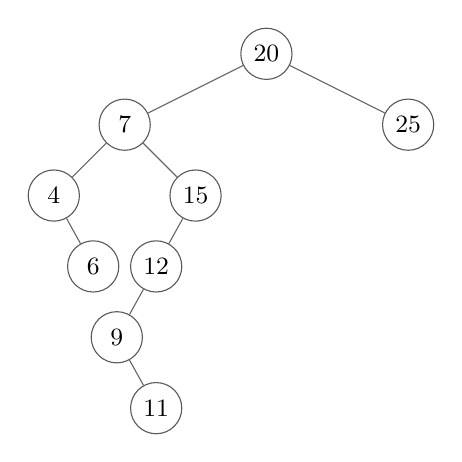
\begin{tikzpicture}[
    btn/.style={circle, draw=black!65, line width=0.4pt, minimum size=6.5mm, inner sep=0pt, font=\small},
    level distance=9mm, edge from parent/.style={draw=black!60},
    level 1/.style={sibling distance=36mm}, level 2/.style={sibling distance=18mm},
    level 3/.style={sibling distance=10mm}, level 4/.style={sibling distance=10mm}]
\node[btn] {20}
    child {node[btn] {7}
        child {node[btn] {4} child[missing] child {node[btn] {6}}}
        child {node[btn] {15}
            child {node[btn] {12}
                child {node[btn] {9} child[missing] child {node[btn] {11}}}
                child[missing]}
            child[missing]}}
    child {node[btn] {25}};
\end{tikzpicture}
\end{center}
檢查：中序是 $4, 6, 7, 9, 11, 12, 15, 20, 25$，由小到大。

\textbf{(b)} 後序（左、右、根）：
\begin{itemize}
\item 7 的左子樹：$4$ 只有右子節點 $6$，得 $6, 4$。
\item 7 的右子樹：$15$ 只有左子樹 $12$；$12$ 只有左子樹 $9$；$9$ 只有右子節點 $11$。 得 $11, 9, 12, 15$。
\item 所以 7 的子樹是 $6, 4, 11, 9, 12, 15, 7$；再接右子樹 $25$ 和根 $20$。
\end{itemize}
後序：$6, 4, 11, 9, 12, 15, 7, 25, 20$。

\textbf{(c)} Top-down 是一個一個插入：放在最後一格，再往上和父節點比，比父節點小就交換（資結書第~8.1~節）。
陣列從 $1$ 開始。
\begin{center}
\small
\begin{tabular}{cll}
\toprule
插入 & 往上冒 & 陣列 \\
\midrule
20 & 根 & 20 \\
7 & $7 < 20$，交換 & 7, 20 \\
15 & $15 > 7$，不動 & 7, 20, 15 \\
4 & 放 $A[4]$；$4 < 20$ 換到 $A[2]$；$4 < 7$ 換到 $A[1]$ & 4, 7, 15, 20 \\
12 & 放 $A[5]$；$12 > 7$，不動 & 4, 7, 15, 20, 12 \\
9 & 放 $A[6]$；$9 < 15$ 換到 $A[3]$；$9 > 4$ 停 & 4, 7, 9, 20, 12, 15 \\
11 & 放 $A[7]$；$11 > 9$，不動 & 4, 7, 9, 20, 12, 15, 11 \\
25 & 放 $A[8]$；$25 > 20$，不動 & 4, 7, 9, 20, 12, 15, 11, 25 \\
6 & 放 $A[9]$；$6 < 20$ 換到 $A[4]$；$6 < 7$ 換到 $A[2]$；$6 > 4$ 停 & 4, 6, 9, 7, 12, 15, 11, 25, 20 \\
\bottomrule
\end{tabular}
\end{center}
最後的最小堆積（陣列 $4, 6, 9, 7, 12, 15, 11, 25, 20$）：
\begin{center}
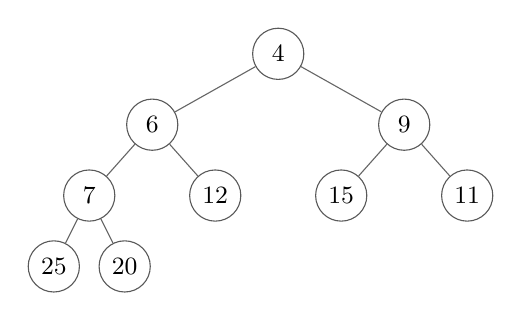
\begin{tikzpicture}[baseline=(current bounding box.north),btn/.style={circle, draw=black!65, line width=0.4pt, minimum size=6.5mm, inner sep=0pt, font=\small},
    level distance=9mm, edge from parent/.style={draw=black!60},
    level 1/.style={sibling distance=32mm}, level 2/.style={sibling distance=16mm}, level 3/.style={sibling distance=9mm}]
\node[btn] {4} child {node[btn] {6} child {node[btn] {7} child {node[btn] {25}} child {node[btn] {20}}} child {node[btn] {12}}} child {node[btn] {9} child {node[btn] {15}} child {node[btn] {11}}};

\end{tikzpicture}
\end{center}

\textbf{(d)} 用最小堆積排成由小到大：反覆刪除根（最小值）並輸出。 刪除的做法是把最後一個元素搬到根，
再往下和比較小的子節點交換，直到不比子節點大（資結書第~8.1~節）。
\begin{center}
\small
\begin{tabular}{clll}
\toprule
次 & 刪除 & 往下調整 & 剩下的堆積 \\
\midrule
1 & 4 & 20 搬到根；和 6 換、和 7 換 & 6, 7, 9, 20, 12, 15, 11, 25 \\
2 & 6 & 25 搬到根；和 7 換、和 12 換 & 7, 12, 9, 20, 25, 15, 11 \\
3 & 7 & 11 搬到根；和 9 換 & 9, 12, 11, 20, 25, 15 \\
4 & 9 & 15 搬到根；和 11 換 & 11, 12, 15, 20, 25 \\
5 & 11 & 25 搬到根；和 12 換、和 20 換 & 12, 20, 15, 25 \\
6 & 12 & 25 搬到根；和 15 換 & 15, 20, 25 \\
7 & 15 & 25 搬到根；和 20 換 & 20, 25 \\
8 & 20 & 25 搬到根 & 25 \\
9 & 25 & & （空） \\
\bottomrule
\end{tabular}
\end{center}
輸出依序是 $4, 6, 7, 9, 11, 12, 15, 20, 25$，由小到大。

若要在同一個陣列裡做（每次把根和堆積最後一格交換、堆積縮小一格），最小堆積會把最小的放到最後面，
陣列變成由大到小；所以「用最小堆積排成由小到大」要照上表依刪除順序輸出（或改用最大堆積就地排序，
資結書第~14.6~節）。 時間 $O(n \log n)$。
\end{pastsoln}
